\documentclass[11pt]{article}
\usepackage[margin=1in]{geometry}
\usepackage{amsmath,amssymb,graphicx,booktabs,longtable}
\usepackage[colorlinks=true,linkcolor=blue,urlcolor=blue]{hyperref}
\usepackage{listings,xcolor}
\lstset{basicstyle=\ttfamily\footnotesize,breaklines=true,frame=single,
  backgroundcolor=\color{gray!8},language=Python,showstringspaces=false}

\title{\textbf{RaoRocketSim}\\[4pt]
\large A Differentiable Rao Thrust-Optimised-Parabola Nozzle Design Tool\\
Reference Manual: Functionality, Mathematics, and Physics}
\author{Ibrahim Shahid}
\date{June 2026 --- J4 gate closed (\texttt{max\_scaled} $= 1.16\times10^{-3} \le 2\times10^{-3}$)}

\begin{document}
\maketitle

\begin{abstract}
RaoRocketSim computes thrust-optimum (Rao/TOP) axisymmetric rocket nozzle
contours by solving Rao's variational problem directly as a discretised
boundary-value problem (BVP), with the method of characteristics (MOC)
supplying the transonic kernel and the wall construction.  The solver is
implemented twice over a single physics definition: a NumPy/SciPy
reference path and a JAX path with \emph{exact} automatic-differentiation
Jacobians solved by Levenberg--Marquardt (Optimistix), held to
$10^{-15}$-level residual parity.  On the reference design point
($\varepsilon=10$, $80\%$ bell, $\gamma=1.4$) the solver converges to
$\max$ scaled residual $1.16\times10^{-3}$ with mass and length
constraints closed to $\mathcal{O}(10^{-9})$, and emits a closed,
monotone wall contour ending exactly on the commanded exit via the NASA
BDE-region construction.  All geometry is \textbf{preliminary design
output}: not CFD-, thermal-, structurally-, or hot-fire-validated.
\end{abstract}

\tableofcontents

%=====================================================================
\section{Repository functionality overview}

\subsection{What the tool does}
Given a design point $(R_t,\ \varepsilon = A_e/A_t,\ \text{length}\,\%,\
\gamma,\ p_a/p_0)$, RaoRocketSim:
\begin{enumerate}
  \item builds the transonic start line TT$'$ (Kliegel--Levine) and
        marches the supersonic \emph{kernel} with axisymmetric MOC;
  \item seeds and solves Rao's variational problem for the optimum
        control surface DE as a coupled residual BVP;
  \item constructs the bell wall from the converged solution via the
        NASA BDE-region march;
  \item exports the contour (CSV / binary STL / plots) and reports a
        residual-backed reliability grade.
\end{enumerate}

\subsection{Module map}
\begin{longtable}{p{0.32\textwidth}p{0.62\textwidth}}
\toprule
\textbf{Module} & \textbf{Responsibility} \\
\midrule
\texttt{raosim/gas\_dynamics.py} & Isentropic ratios, Prandtl--Meyer
function and inverse, Mach angle, area--Mach relation, critical Mach
$M^*$, ideal thrust coefficient. \\
\texttt{raosim/moc.py} & Axisymmetric MOC unit processes (interior,
axis, wall points), characteristic-net marching, compatibility
auditing.\\
\texttt{raosim/transonic\_kernel.py} & Mathematically corrected
Kliegel--Levine third-order transonic evaluator. \\
\texttt{raosim/nasa\_moc.py} & Port of the NASA/JHU
\texttt{MOC\_GridCalc\_BDE.cpp} workflow: \texttt{KLThroat} (visible-source
semantics), \texttt{CalcInitialThroatLine}, RRC kernel march
(\texttt{build\_kernel}), \texttt{CalcMdotBD}, \texttt{FindPointE},
\texttt{CalcLRCDE} (free-exit and FIXEDEND branches), \texttt{SetThetaB},
BDE-region wall (\texttt{calc\_bde\_region}). Oracle-validated against the
checked-in \texttt{outputs\_M3.5Perf} reference grids. \\
\texttt{raosim/rao\_variational.py} & The Rao BVP: configuration,
unknown packing, residual blocks (legacy and \emph{characteristic}
formulations), seeding, the solve shell, wall construction dispatch,
reliability ladder. \\
\texttt{raosim/jax/} & Differentiable backend: \texttt{primitives}
(J1-parity gas dynamics), \texttt{residuals} (vectorised leaves),
\texttt{assembly} (full residual, $10^{-15}$ parity), \texttt{bvp}/
\texttt{api} (Optimistix LM, sigmoid-bounded, constraint-weight ladder). \\
\texttt{raosim/nozzle\_geometry.py} & Chart-calibrated B\'ezier Rao/TOP
approximation (published $\theta_N,\theta_E$ tables); conical nozzles. \\
\texttt{raosim/export.py, plotting.py, trajectory.py, \ldots} &
CSV/STL export, plots, altitude performance, trade studies, CLI. \\
\texttt{scripts/generate\_contour.py} & Parametric end-to-end generator
(\S\ref{sec:generator}). \\
\texttt{scripts/j4\_report.py} & One-shot solver status report. \\
\bottomrule
\end{longtable}

%=====================================================================
\section{Governing gas dynamics}
Calorically perfect, inviscid, irrotational, axisymmetric flow with
stagnation-normalised state ($p/p_0$, $T/T_0$, $\rho/\rho_0$).

\subsection{Isentropic relations}
\begin{equation}
\frac{T_0}{T} = 1+\frac{\gamma-1}{2}M^2,\qquad
\frac{p}{p_0}=\Big(\frac{T}{T_0}\Big)^{\frac{\gamma}{\gamma-1}},\qquad
\frac{\rho}{\rho_0}=\Big(\frac{T}{T_0}\Big)^{\frac{1}{\gamma-1}}.
\end{equation}

\subsection{Prandtl--Meyer function and Mach angle}
\begin{equation}
\nu(M)=\sqrt{\tfrac{\gamma+1}{\gamma-1}}
\arctan\!\sqrt{\tfrac{\gamma-1}{\gamma+1}(M^2-1)}-\arctan\!\sqrt{M^2-1},
\qquad \mu = \arcsin(1/M).
\end{equation}

\subsection{Critical Mach number}
\begin{equation}
M^{*2} = \frac{(\gamma+1)M^2}{2+(\gamma-1)M^2},
\end{equation}
the velocity normalised by the throat speed of sound; it appears in
Rao's algebraic stationarity (\S\ref{sec:rao}).

\subsection{Area--Mach relation}
\begin{equation}
\frac{A}{A^*}=\frac{1}{M}\Big[\frac{2}{\gamma+1}
\Big(1+\frac{\gamma-1}{2}M^2\Big)\Big]^{\frac{\gamma+1}{2(\gamma-1)}} .
\end{equation}

%=====================================================================
\section{Method of characteristics (axisymmetric)}
\label{sec:moc}
Characteristic directions $dr/dx=\tan(\theta\pm\mu)$ ($C^\pm$).
Compatibility along them (Anderson, \emph{Modern Compressible Flow},
Ch.~11):
\begin{equation}
d(\theta+\nu) = Q^{+}\,ds \ \ \text{on } C^{+},\qquad
d(\theta-\nu) = Q^{-}\,ds \ \ \text{on } C^{-},
\end{equation}
\begin{equation}
Q^{\pm} = \pm\,\frac{\sin\theta\,\sin\mu\,\cos\mu}{r\,\cos(\theta\pm\mu)} .
\end{equation}
The axisymmetric source terms $Q^\pm$ make $\theta\pm\nu$ \emph{local}
quantities, not global invariants.  Unit processes (interior, axis,
wall) solve the two-equation system per node; the NASA port uses the
d$\theta$-form derivative system of \texttt{MOC\_GridCalc\_BDE.cpp}.

\subsection{Transonic start line (Kliegel--Levine)}
The kernel cannot start at $M=1$ exactly; the TT$'$ line comes from the
third-order Kliegel--Levine expansion in inverse powers of
$(R_u/R_t+1)$, where $R_u$ is the \emph{upstream} wall radius of
curvature (Hall 1962; Kliegel \& Levine 1969).  Two port subtleties are
load-bearing and oracle-pinned by
\texttt{tests/test\_nasa\_kernel\_march\_parity.py}:
\begin{itemize}
  \item \textbf{C++ integer division}: the visible source computes
  $z\,(y^2-5/8)$ with \texttt{5/8}$\,=0$; the binary that generated all
  reference fixtures ran with the term dropped.  The ``visible-source''
  evaluator reproduces this exactly (TT$'$ matches \texttt{TT'.out} to
  $5\times10^{-7}$); the theory-correct $y^2-5/8$ lives in
  \texttt{transonic\_kernel.py}.
  \item \textbf{Upstream radius}: \texttt{CalcInitialThroatLine(rUp,..)}
  feeds the \emph{upstream} radius into KLThroat.  Rao convention:
  $R_u=1.5R_t$ upstream, $R_d=0.382R_t$ downstream
  (\texttt{throat\_upstream\_radius\_factor}).
\end{itemize}
With both honoured, \texttt{build\_kernel} reproduces NASA's M3.5Perf
kernel: 58 RRC rows, BD matching \texttt{LastKernel.out} node for node.

%=====================================================================
\section{Rao's variational problem}
\label{sec:rao}
Rao (1958) maximises thrust over exit contours of fixed length and area
ratio.  The optimum is characterised on a \emph{control surface} DE --- a
left-running ($C^{+}$) characteristic from a kernel point D to the exit
lip E --- by integrals of the flow:
\begin{align}
F &= \int_{DE} 2\pi r\Big[\rho V^2 \cos\theta\,
      \frac{\sin(\phi-\theta)}{\sin\phi} + (p-p_a)\Big]\,dr
      &&\text{(thrust)},\\
\dot m &= \int_{DE} 2\pi r\,\rho V\,\frac{\sin(\phi-\theta)}{\sin\phi}\,dr
      &&\text{(mass flow)},\\
L &= z_C + \int_{DE} \cot\phi\, dr
      &&\text{(\textbf{exit station}; } z_C = x_D\text{)} .
\end{align}
The Euler--Lagrange conditions collapse to the \emph{algebraic Rao
stationarity} (Rao--Beck--Booth, AIAA 99-2584, Eq.~3):
\begin{equation}
\boxed{\ \frac{M^{*}\cos(\theta-\alpha)}{\cos\alpha} = C
\quad\text{constant along DE},\qquad \alpha=\arcsin(1/M).\ }
\label{eq:stationarity}
\end{equation}
Mass closure ties DE to the kernel: the flux crossing DE equals the
flux crossing the kernel characteristic segment B$\to$D,
\begin{equation}
\dot m_{DE} \;=\; \dot m_{BD},\qquad
\dot m_{\Gamma} = \int_{\Gamma} 2\pi r\,\rho V\,
|\sin(\beta-\theta)|\,ds ,
\label{eq:mass}
\end{equation}
with $\beta$ the local polyline tangent.  The smooth optimum exists
only inside Guderley's validity region; the solver checks the
inequality (\texttt{rao\_valid\_region}) and reports
\texttt{requires\_discontinuous\_exit\_flow\_model} otherwise.

\paragraph{Length bookkeeping (a load-bearing correction).}
The constraint is the \emph{exit station} $x_E = z_C + \int\cot\phi\,dr$.
An earlier implementation compared $\sum dx = x_E - x_D$ against $L$
while a separate residual pinned $x_E=L$ --- contradictory unless
$x_D\to0$, which silently drove the solved D to the throat plane.
Restoring $z_C$ moved the reference solve from
$\max$ scaled $6.2\times10^{-2}$ to $3.0\times10^{-3}$ in one step.

%=====================================================================
\section{NASA topology constructions}
Ports of \texttt{MOC\_GridCalc\_BDE.cpp} (Rice, JHU/APL 2003):
\begin{description}
  \item[\texttt{CalcMdotBD}] mass flux from B to a candidate D along the
  kernel's final RRC (annular trapezoids of $\rho u$).
  \item[\texttt{FindPointE}] integrates the $C^{+}$ derivative system
  (RKF45 in $r$) from D, accumulating annular mass until
  $\dot m_{DE}=\dot m_{BD}$; the terminus is E.
  \item[\texttt{CalcLRCDE}] places D on BD.  Two inner conditions:
  \emph{free-exit} (\texttt{rao\_free}) zeroes
  $\theta_E-\tfrac12\arcsin\!\big[2(p_E-p_a)/(\rho_E V_E^2\tan\mu_E)\big]$
  (Rao Eq.~14); \emph{FIXEDEND} (\texttt{fixed\_end}) walks D until
  $r_E$ crosses the commanded exit radius, then secants.  The fixed-$
  (L,\varepsilon)$ design point uses FIXEDEND.
  \item[\texttt{SetThetaB}] outer secant on the initial expansion angle
  $\theta_B$ driving the remaining exit parameter (length), with
  SEC\_FAIL-style bracketing.  Note the monotonicity: \emph{lower}
  $\theta_B$ $\Rightarrow$ \emph{longer} nozzle.
  \item[\texttt{calc\_bde\_region}] back-computes the region bounded by
  BD, DE and the wall, then locates each wall point by mass
  conservation (\texttt{CalcWallContour}) --- this is the wall used by
  \texttt{wall\_method="bde"}.
\end{description}

%=====================================================================
\section{The BVP formulation}
\subsection{Unknowns}
\begin{equation}
u = \big[\,M_{1..n},\ \theta_{1..n},\ r_{1..n}\ \big|\
\lambda_2,\ \lambda_3,\ \log C,\ f_D\,\big],
\end{equation}
where $f_D\in[0,1]$ is D's arc-length fraction along the (static)
kernel BD.  $x$ is \emph{reconstructed}, not carried: DE is a $C^{+}$
characteristic by construction,
\begin{equation}
x_{i+1} = x_i + \frac{\Delta r}{\tan(\bar\theta+\bar\mu)},\qquad
x_1 = x_D(f_D),
\end{equation}
making left-Mach geometry exact to machine precision.

\subsection{Residual blocks (characteristic formulation)}
\begin{center}
\begin{tabular}{lll}
\toprule
block & content & scaling \\
\midrule
\texttt{mass} & $(\dot m_{DE}-\dot m_{BD})/\dot m_{\mathrm{ref}}$ & relative \\
\texttt{length} & $(x_E - L)/L$ \quad (exit station) & relative \\
\texttt{algebraic\_stationarity} & $\log M^* + \log|\cos(\theta-\alpha)|$ & per node \\
 & $\ -\log\cos\alpha-\log C$ & \\
\texttt{moc\_cplus} & $\Delta(\theta+\nu) - Q^{+}\Delta s$ per segment & $/1^\circ$ \\
\texttt{ce\_geometry} & D attachment ($r$ pin; optional $\theta$, $M$ pins), & mixed \\
 & exit pin $(x_E,r_E)=(L,R_e)$, monotonicity & \\
\texttt{regularization} & $0.02\,\Delta^2(\theta\pm\nu)$ & $/1^\circ$ \\
\texttt{penalties} & one-sided monotonicity guards & --- \\
\bottomrule
\end{tabular}
\end{center}
Deliberately \emph{absent} relative to the legacy stack (each removal
literature-grounded and empirically decisive):
\texttt{moc\_cminus} on DE (the $C^{-}$ relation does not hold along a
$C^{+}$ characteristic; Rao's closure carries only $C^{+}$ relations
$+$ stationarity $+$ integrals) and the CE$\to$wall $C^{+}$ pairing
blocks (the $C^{+}$ through a DE point \emph{is} DE; the wall belongs
to the BDE region).  The D attachment is position-only at the gate
(\texttt{pin\_d\_theta=False}): pinning $\theta_1$ to the
\emph{interpolated, approximate} kernel angle imports kernel
discretisation error into the stationarity chain at full weight.

%=====================================================================
\section{The differentiable (JAX) backend}
The entire residual is re-expressed in \texttt{jax.numpy}
(\texttt{raosim/jax/assembly.py}) and held to $\sim10^{-15}$ parity with
the NumPy assembly on real solver states (J2 gate).  The solve is
Levenberg--Marquardt (Optimistix) with \emph{exact} \texttt{jacfwd}
Jacobians --- replacing SciPy's finite-difference Jacobian, whose noise
near the sonic and Mach-line singularities was the original convergence
suspect.  Box bounds are enforced by a smooth sigmoid reparametrisation
$u = \ell + (h-\ell)\,\sigma(z)$, and the integral constraints
(single residual elements vs.\ $\mathcal{O}(n)$ physics elements) are
up-weighted along a continuation ladder $(1,10,30,100)$, each rung
warm-starting the next; reported residuals are always unweighted.

\begin{lstlisting}
cfg = RaoSolverConfig(
    Rt=0.020, epsilon=10.0, gamma=1.4, pa_over_p0=0.01, length_pct=80.0,
    n_control=24, n_kernel=24, max_nfev=4000, residual_tol=2e-3,
    evaluate_moc=True, wall_method="bde",
    solver_backend="jax", formulation="characteristic",
    pin_d_theta=False, thetaN_guess_deg=21.87,
    jax_constraint_weight_ladder=(1.0, 10.0, 30.0, 100.0))
sol = solve_rao_bvp(cfg)   # sol.residuals.max_scaled -> 1.16e-3
\end{lstlisting}

%=====================================================================
\section{Convergence campaign (the J4 record)}
\begin{center}
\begin{tabular}{lll}
\toprule
$\max$ scaled & change introduced & root cause closed \\
\midrule
$\approx 8$ & (baseline) SciPy FD Jacobian & --- \\
$2.8$ & exact-Jacobian LM (JAX) & FD noise removed \\
$0.50$ & KLThroat int-division $+$ $R_u$ fixes & kernel march never ran \\
$0.49$ & NASA FIXEDEND topology seed & degenerate D$\approx$E seed \\
$0.062$ & characteristic formulation $+$ ladder & $C^-$-on-$C^+$ scaffolds \\
$0.0030$ & exit-station length ($z_C$ restored) & $x_D$ double-count \\
$\mathbf{0.00116}$ & position-only D attachment & $\theta_D$ interpolation error \\
\bottomrule
\end{tabular}
\end{center}
At the gate: mass $-1.9\times10^{-9}$, length $-5.8\times10^{-10}$,
$f_D=0.304$ (the classical interior band), $\theta_B = 21.87^\circ$
--- independently recovering the published chart angle
$\theta_N(\varepsilon{=}10, 80\%)\approx21.9^\circ$.

%=====================================================================
\section{Parametric contour generation}
\label{sec:generator}
\texttt{scripts/generate\_contour.py} is the end-to-end entry point:
\begin{lstlisting}[language=bash]
PYTHONPATH=. python scripts/generate_contour.py \
    --rt 0.020 --epsilon 10 --length-pct 80 --gamma 1.4 \
    --theta-b-guess 21.87 --out builds/my_nozzle
\end{lstlisting}
It refuses to export unless the $2\times10^{-3}$ gate passes (override
with \texttt{--allow-unconverged}) and writes \texttt{contour.csv},
a binary \texttt{contour\_3d.stl} surface of revolution, and the two
figures below.

\begin{figure}[h!]
\centering
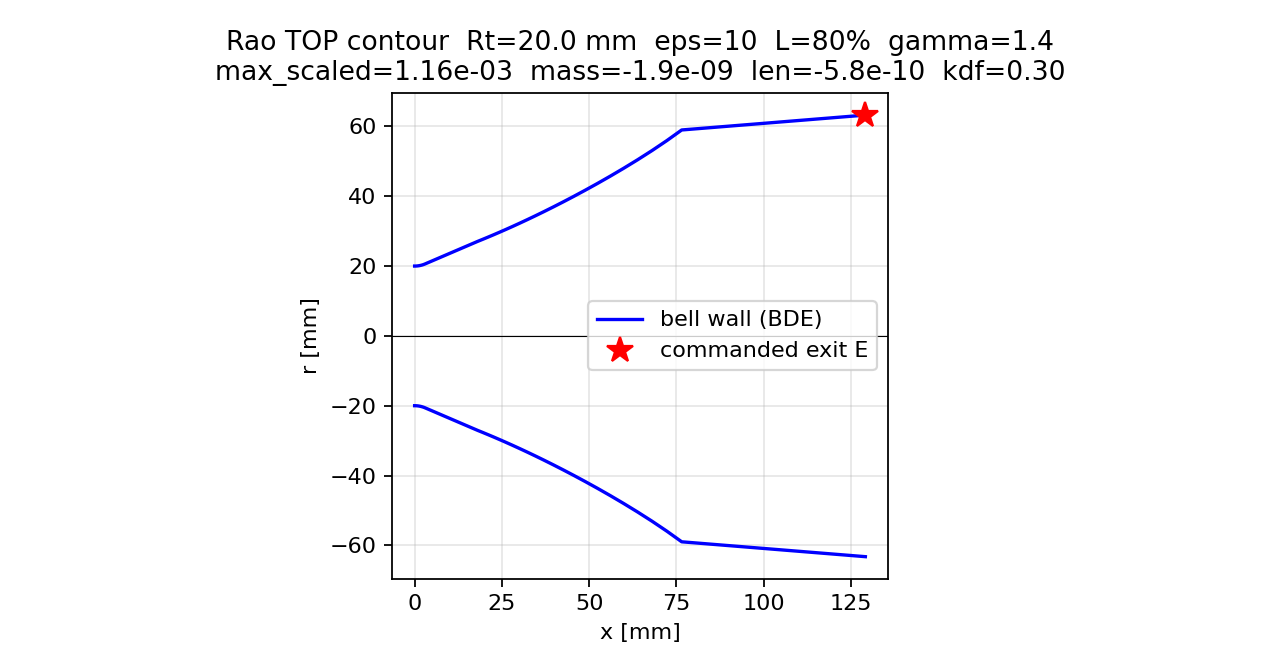
\includegraphics[width=0.95\textwidth]{figures/ref_run/contour.png}
\caption{Converged Rao TOP profile for the reference design point
($R_t=20$\,mm, $\varepsilon=10$, $80\%$, $\gamma=1.4$).  The wall is the
NASA BDE-region construction from the \emph{solved} control surface;
its final point lands exactly on the commanded exit (star).}
\end{figure}

\begin{figure}[h!]
\centering
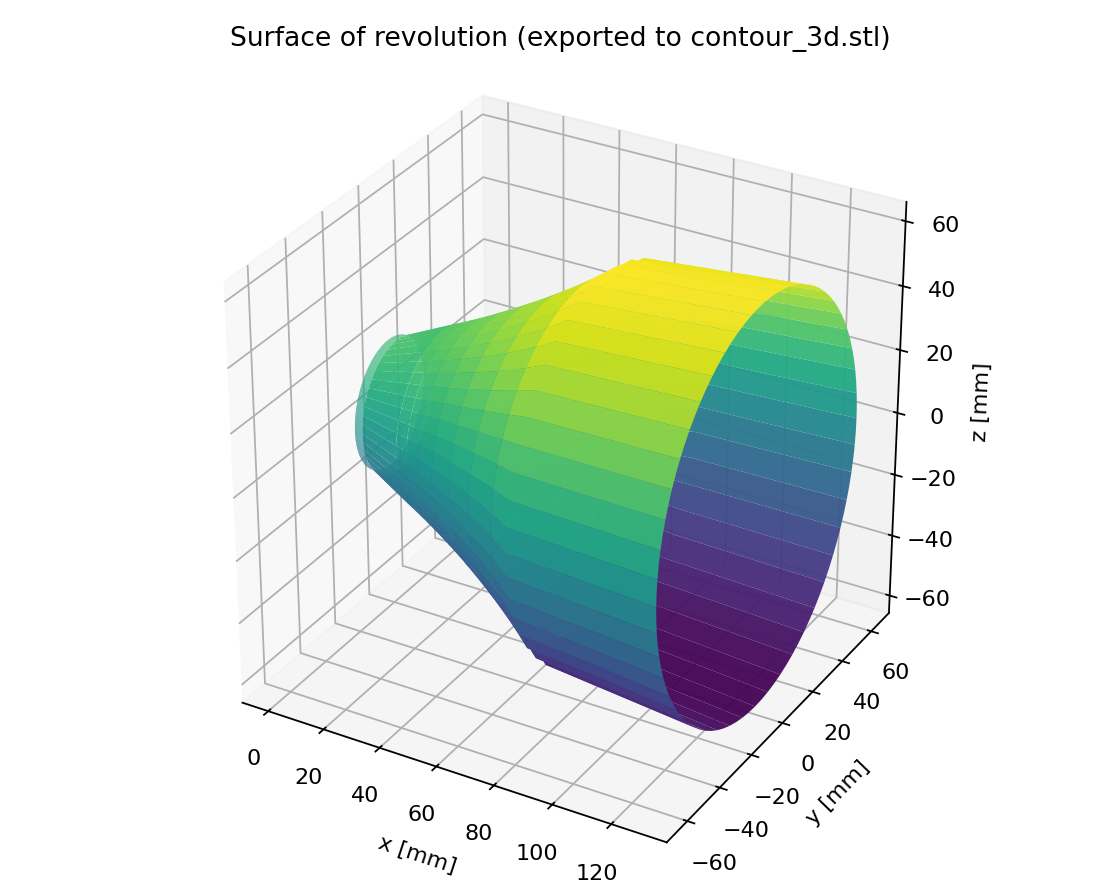
\includegraphics[width=0.72\textwidth]{figures/ref_run/contour_3d.png}
\caption{Surface of revolution of the same contour (exported as binary
STL for CAD/printing).}
\end{figure}

%=====================================================================
\section{Verification and reliability}
\begin{itemize}
  \item \textbf{Oracle parity}: kernel march vs.\ NASA M3.5Perf grids
  (TT$'$ $5\times10^{-7}$; full 58-row grid; BD vs
  \texttt{LastKernel.out}).
  \item \textbf{Backend parity}: JAX vs NumPy residual $\sim10^{-15}$
  on real states; \texttt{jacfwd}$=$\texttt{jacrev}$=$central differences.
  \item \textbf{Gates}: J4 ($\max$ scaled $\le2\times10^{-3}$) and the
  closed-wall test are ordinary (non-xfail) tests in
  \texttt{tests/test\_jax\_convergence.py}.
  \item \textbf{Reliability ladder}: \texttt{GEOMETRIC\_APPROXIMATION}
  $\to$ \texttt{MOC\_COMPATIBLE} $\to$
  \texttt{RAO\_VARIATIONAL\_RESIDUAL\_SOLVED} $\to$
  \texttt{BENCHMARK\_VALIDATED}; promotion past the first grade is
  currently held by the forward-MOC audit alignment (below).
  \item \textbf{Caveats}: every output carries
  \texttt{hardware\_qualified=False}.  No CFD, thermal, structural,
  manufacturing, or hot-fire validation is implied.
\end{itemize}

%=====================================================================
\section{Remaining roadmap (formalised final steps)}
\begin{enumerate}
  \item \textbf{Default flip + re-baseline}: make
  \texttt{formulation="characteristic"}, \texttt{pin\_d\_theta=False},
  the ladder, and \texttt{wall\_method="bde"} the defaults; re-baseline
  the Phase-6/7 test expectations on the converged numbers.
  \item \textbf{Forward-MOC audit alignment}: the verification pass
  still marches a spline wall from a chart-$\theta_N$ start line;
  align it with BDE-built walls so \texttt{moc\_ok} can promote
  reliability honestly.
  \item \textbf{J5 chart sweep}: run the converged configuration across
  the $(\varepsilon, \text{length}\%)$ grid against the published
  $\theta_N/\theta_E$ tables (targets: RMS $1.5^\circ$, max $3^\circ$)
  --- the \texttt{BENCHMARK\_VALIDATED} gate.
  \item \textbf{J6 gradient API}: \texttt{rao\_sensitivities} ---
  $\partial C_f/\partial(\text{params})$ and the per-node
  $|\partial C_f/\partial r_i|$ manufacturing-tolerance field via
  implicit differentiation through the converged LM solve (machinery
  already proven in \texttt{tests/test\_jax\_bvp.py}).
  \item \textbf{Phase 12.4 march robustness}: extend the kernel past the
  $\theta_B\approx24^\circ$ unit-process edge (tight throats), which
  also unlocks full state continuity at D (\texttt{pin\_d\_mach}).
  \item \textbf{J3b}: \texttt{lax.scan} port of the march, making
  $\theta_B$ a solved unknown and enabling kernel-parameter
  sensitivities (start-line provenance studies).
\end{enumerate}

%=====================================================================
\begin{thebibliography}{9}
\bibitem{rao58} G.~V.~R. Rao, ``Exhaust Nozzle Contour for Optimum
Thrust,'' \emph{Jet Propulsion} 28(6), 1958.
\bibitem{rao99} G.~V.~R. Rao, J.~Beck, T.~Booth, ``Nozzle Optimization
for Space-Based Vehicles,'' AIAA 99-2584, 1999.
\bibitem{rice03} T.~Rice, \emph{2-D/Axisymmetric MOC Nozzle Design
Code}, JHU/APL RTDC-TPS-481, 2003 (visible source:
\texttt{MOC\_GridCalc\_BDE.cpp}).
\bibitem{kl69} J.~R. Kliegel, J.~N. Levine, ``Transonic Flow in Small
Throat Radius of Curvature Nozzles,'' \emph{AIAA J.} 7(7), 1969.
\bibitem{hall62} I.~M. Hall, ``Transonic Flow in Two-Dimensional and
Axially-Symmetric Nozzles,'' \emph{QJMAM} 15(4), 1962.
\bibitem{anderson} J.~D. Anderson, \emph{Modern Compressible Flow},
3rd ed., Ch.~11.
\bibitem{ostlund} J.~\"Ostlund, \emph{Flow Processes in Rocket Engine
Nozzles with Focus on Flow Separation and Side-Loads}, KTH, 2002.
\bibitem{guderley} K.~G. Guderley et al., ``Continuous and
discontinuous solutions for optimum thrust nozzles of given length,''
\emph{JOTA}, 1968.
\bibitem{optimistix} J.~Rader, T.~Lyons, P.~Kidger, ``Optimistix,''
arXiv:2402.09983.
\end{thebibliography}

\end{document}
